\RequirePackage[l2tabu, orthodox]{nag}
\RequirePackage{silence}
  \WarningFilter{biblatex}{Patching footnotes failed}
%   \WarningFilter{hyperref}{Option `pdflang' has already been used}
%   \WarningFilter{hyperref}{Option `pdfdisplaydoctitle' has already been used}
  \WarningFilter{hyperref}{Token not allowed in a PDF string}
  \WarningFilter{biblatex}{Field 'prefixnumber' deprecated.}
  \WarningFilter{Fancyhdr}{\headheight is too small}

\documentclass[sigconf,natbib=false,anonymous=false]{acmart}

%%% Subliminal refinements towards typographical perfection (1%)
% \usepackage[stretch=10]{microtype}

%drt24 hacks
% Letter paper
\setlength{\paperheight}{11in}
\setlength{\paperwidth}{8.5in}

%%% Handle input and output of accented/special characters and modern fonts
\usepackage[T1]{fontenc}
\usepackage[utf8]{inputenc}
\usepackage{lmodern}

%%% Better biblatex
\let\citename\relax
\usepackage[american]{babel}
\usepackage{csquotes}
\usepackage[style=ACM-Reference-Format,
  abbreviate=true, dateabbrev=true, isbn=true, doi=true, urldate=comp, url=true, eprint=false,
  maxbibnames=9, minbibnames=9, maxcitenames=1, mincitenames=1,
  backref=false, backend=biber, language=american, sortcites=true,
  autocite=inline% , labelnumber=true
  ]{biblatex}
% \cite, \parencite, \footcite, \textcite, \autocite

\setcounter{biburlnumpenalty}{100}
\setcounter{biburllcpenalty}{9000}

\addbibresource{references/refs.bib}
\renewcommand{\bibfont}{\Small}

%%% Include todo notes while writing draft (\listoftodos, \todo, \missingfigure)
\usepackage[color=white]{todonotes}

%%% Demo boxes
\usepackage{xcolor}
\newcommand\crule[3][black]{\textcolor{#1}{\rule{#2}{#3}}}

%%% Easier SI units
\usepackage[allowlitunits]{siunitx}

%%% Improved subfigures
% \usepackage[caption=false,font=footnotesize]{subfig}
\usepackage[caption=false,font=footnotesize]{subfig}
\usepackage[export]{adjustbox}

\usepackage{float}


%%% Better looking tables
\usepackage{booktabs}
\renewcommand{\arraystretch}{1.2}
\usepackage{array}


%%% Better handling of links
\usepackage{url}


%%% Better math
\usepackage{amsmath}


%%% Colors for tracking changes
\newcommand{\red}[1]{\textcolor{red}{#1}}
\newcommand{\blue}[1]{\textcolor{blue}{#1}}

% \usepackage{setspace}
% \doublespacing


%%% JSON Listing
\usepackage{listings}
\newcommand\JSONnumbervaluestyle{\color{blue}}
\newcommand\JSONstringvaluestyle{\color{red}}
% switch used as state variable
\newif\ifcolonfoundonthisline

\makeatletter

\lstdefinestyle{json}
{
  showstringspaces    = false,
  keywords            = {false,true},
  alsoletter          = 0123456789.,
  morestring          = [s]{"}{"},
  stringstyle         = \ifcolonfoundonthisline\JSONstringvaluestyle\fi,
  MoreSelectCharTable =%
    \lst@DefSaveDef{`:}\colon@json{\processColon@json},
  basicstyle          = \ttfamily,
  keywordstyle        = \ttfamily\bfseries,
}

% flip the switch if a colon is found in Pmode
\newcommand\processColon@json{%
  \colon@json%
  \ifnum\lst@mode=\lst@Pmode%
    \global\colonfoundonthislinetrue%
  \fi
}

\lst@AddToHook{Output}{%
  \ifcolonfoundonthisline%
    \ifnum\lst@mode=\lst@Pmode%
      \def\lst@thestyle{\JSONnumbervaluestyle}%
    \fi
  \fi
  %override by keyword style if a keyword is detected!
  \lsthk@DetectKeywords%
}

% reset the switch at the end of line
\lst@AddToHook{EOL}%
  {\global\colonfoundonthislinefalse}

\makeatother



%%% Commands for easily changing formatting (e.g., italicize)
\newcommand{\etal}{et~al.}
\newcommand{\ie}{i.e.}
\newcommand{\eg}{e.g.}

\newcommand{\figref}[1]{Figure~\ref{#1}}
\newcommand{\tblref}[1]{Table~\ref{#1}}
\newcommand{\secref}[1]{Section~\ref{#1}}


% Removes citation information below abstract
% \settopmatter{printacmref=false}


\begin{document}

\title{Review: A Web-Based Simulation Viewer for Sharing\\Evolutionary Robotics Results}

\author{Anthony J. Clark}
\affiliation{%
  \institution{Computer Science Department\\Missouri State University}
  \city{Springfield}
  \state{Missouri}
  \country{USA}
}
\email{anthonyclark@missouristate.edu}


\author{Jared M. Moore}
\affiliation{%
  \institution{School of Computing and Information Systems\\Grand Valley State University}
  \city{Allendale}
  \state{Michigan}
  \country{USA}
}
\email{moorejar@gvsu.edu}


% Maximum 200 words

\begin{abstract}

%%% Background
% This section should be the shortest part of the abstract and should very briefly outline the following information:
% - What is already known about the subject, related to the paper in question
% - What is not known about the subject and hence what the study intended to examine (or what the paper seeks to present)
Evolutionary robotics researchers often need to share results that may be too difficult to describe in text and too complex to show using images. Many researchers include links to videos as supplementary materials, but videos have a predefined view of the scene and do not allow watchers to adjust the viewing angle to their preference.
%
%
%
%%% Methods
% The methods section is usually the second-longest section in the abstract. It should contain enough information to enable the reader to understand what was done, and how.
In this paper we present a web-based application (based on three.js) for sharing interactive animations. Specifically, our tool (called Review) enables researchers to generate simple animation log data that can be loaded in any modern web browser on a computer or mobile device. The camera in these animations can be controlled by the user such that they can pan, tilt, rotate, and zoom in and out of the scene.
%
%
%
% Results
% The results section should be the longest part of the abstract and should contain as much detail about the findings as the journal word count permits.
%
%
%
% Conclusion
% This section should contain the most important take-home message of the study, expressed in a few precisely worded sentences. Usually, the finding highlighted here relates to the primary outcome measure; however, other important or unexpected findings should also be mentioned. It is also customary, but not essential, for the authors to express an opinion about the theoretical or practical implications of the findings, or the importance of their findings for the field. Thus, the conclusions may contain three elements:
% - The primary take-home message
% - The additional findings of importance
% - The perspective
Review is meant to improve the ability of researchers to share their evolved results with one another.

\end{abstract}

% Evolutionary robotics researchers often need to share results that may be too difficult to describe in text and too complex to show using images. Many researchers include links to videos as supplementary materials, but videos have a predefined view of the scene and do not allow watchers to adjust the viewing angle to their preference. In this paper we present a web-based application (based on three.js) for sharing interactive animations. Specifically, our tool (called Review) enables researchers to generate simple animation log data that can be loaded in any modern web browser on a computer or mobile device. The camera in these animations can be controlled by the user such that they can pan, tilt, rotate, and zoom in and out of the scene. Review is meant to improve the ability of researchers to share their evolved results with one another.


%
% The code below should be generated by the tool at
% http://dl.acm.org/ccs.cfm
% Please copy and paste the code instead of the example below.
%
\begin{CCSXML}
<ccs2012>
<concept>
<concept_id>10010147.10010341.10010349.10010364</concept_id>
<concept_desc>Computing methodologies~Scientific visualization</concept_desc>
<concept_significance>500</concept_significance>
</concept>
<concept>
<concept_id>10010147.10010257.10010293.10011809.10011814</concept_id>
<concept_desc>Computing methodologies~Evolutionary robotics</concept_desc>
<concept_significance>300</concept_significance>
</concept>
</ccs2012>
\end{CCSXML}

\ccsdesc[500]{Computing methodologies~Scientific visualization}
\ccsdesc[300]{Computing methodologies~Evolutionary robotics}


\copyrightyear{2018}
\acmYear{2018}
\setcopyright{acmlicensed}
\acmConference[GECCO '18 Companion]{Genetic and Evolutionary Computation Conference Companion}{July 15--19, 2018}{Kyoto, Japan}
\acmBooktitle{GECCO '18 Companion: Genetic and Evolutionary Computation Conference Companion, July 15--19, 2018, Kyoto, Japan}
\acmPrice{15.00}
\acmDOI{10.1145/3205651.3208292}
\acmISBN{978-1-4503-5764-7/18/07}

% \CopyrightYear{2018}
% \setcopyright{acmlicensed}
% \conferenceinfo{GECCO '18 Companion,}{July 15--19, 2018, Kyoto, Japan}
% \isbn{978-1-4503-5764-7/18/07}\acmPrice{$15.00}
% \doi{https://doi.org/10.1145/3205651.3208292}


\keywords{evolutionary robotics, visualization}

\maketitle

\section{Introduction}

% (1) Introductory paragraph: Very briefly: What is the problem and why is it relevant to the audience attending *THIS CONFERENCE*? Moreover, why is the problem hard, and what is your solution? You must be brief here. This forces you to boil down your contribution to its bare essence and communicate it directly.
Conveying the behaviors of a dynamic system is extremely important in the field of robotics.
%
When presenting the operation of a new robotic system, it is vital to provide readers and collaborators with some way to visualize its motions.
%
This is particularly true for evolutionary robotics (ER) research, as
%
often the goal of ER is to produce \emph{novel} or unexpected behaviors.
%
Despite this importance, however, it can be difficult to present behaviors in a manner useful to other researchers.
%
In this paper, we present \textbf{Review}\footnote{https://review.github.io/} (source code\footnote{\url{https://github.com/review/review.github.io}}), a web-based platform for sharing visualizations of evolved robotic systems.




% (2) Background paragraph: Elaborate on why the problem is hard, critically examining prior work, trying to tease out one or two central shortcomings that your solution overcomes.
Traditionally, to depict behaviors of an evolved system, researchers provide sequences of images (see Figures~\ref{fig:quad_gaits} and~\ref{fig:worm_gaits}) and/or links to videos.
%
Image sequences have been a common feature of ER from the beginning; see, \textcite{Sims.1994.CGIT.Creatures} from \citeyear{Sims.1994.CGIT.Creatures} for example.
%
Images, however, can sometimes be problematic. First, when a reader is unfamiliar with terminology (\eg{}, gait, hopping, bounding, etc.) they may not have a baseline reference with which to compare and understand images of a new behavior.
%
And second, even with a good understanding of what to expect, some complex movements are difficult to comprehend from image sequences.
%
For example, the quadruped gaits in Figure~\ref{fig:quad_gaits} are reasonably understandable for someone familiar with such systems, but for someone new to quadrupedal robotics it may be difficult to picture the motions.
%
Likewise, the unusual gaits exhibited by the worm-like animat in Figure~\ref{fig:worm_gaits} are difficult to imagine without the aid of video (or animation).



\begin{figure*}[htb!]
\centering
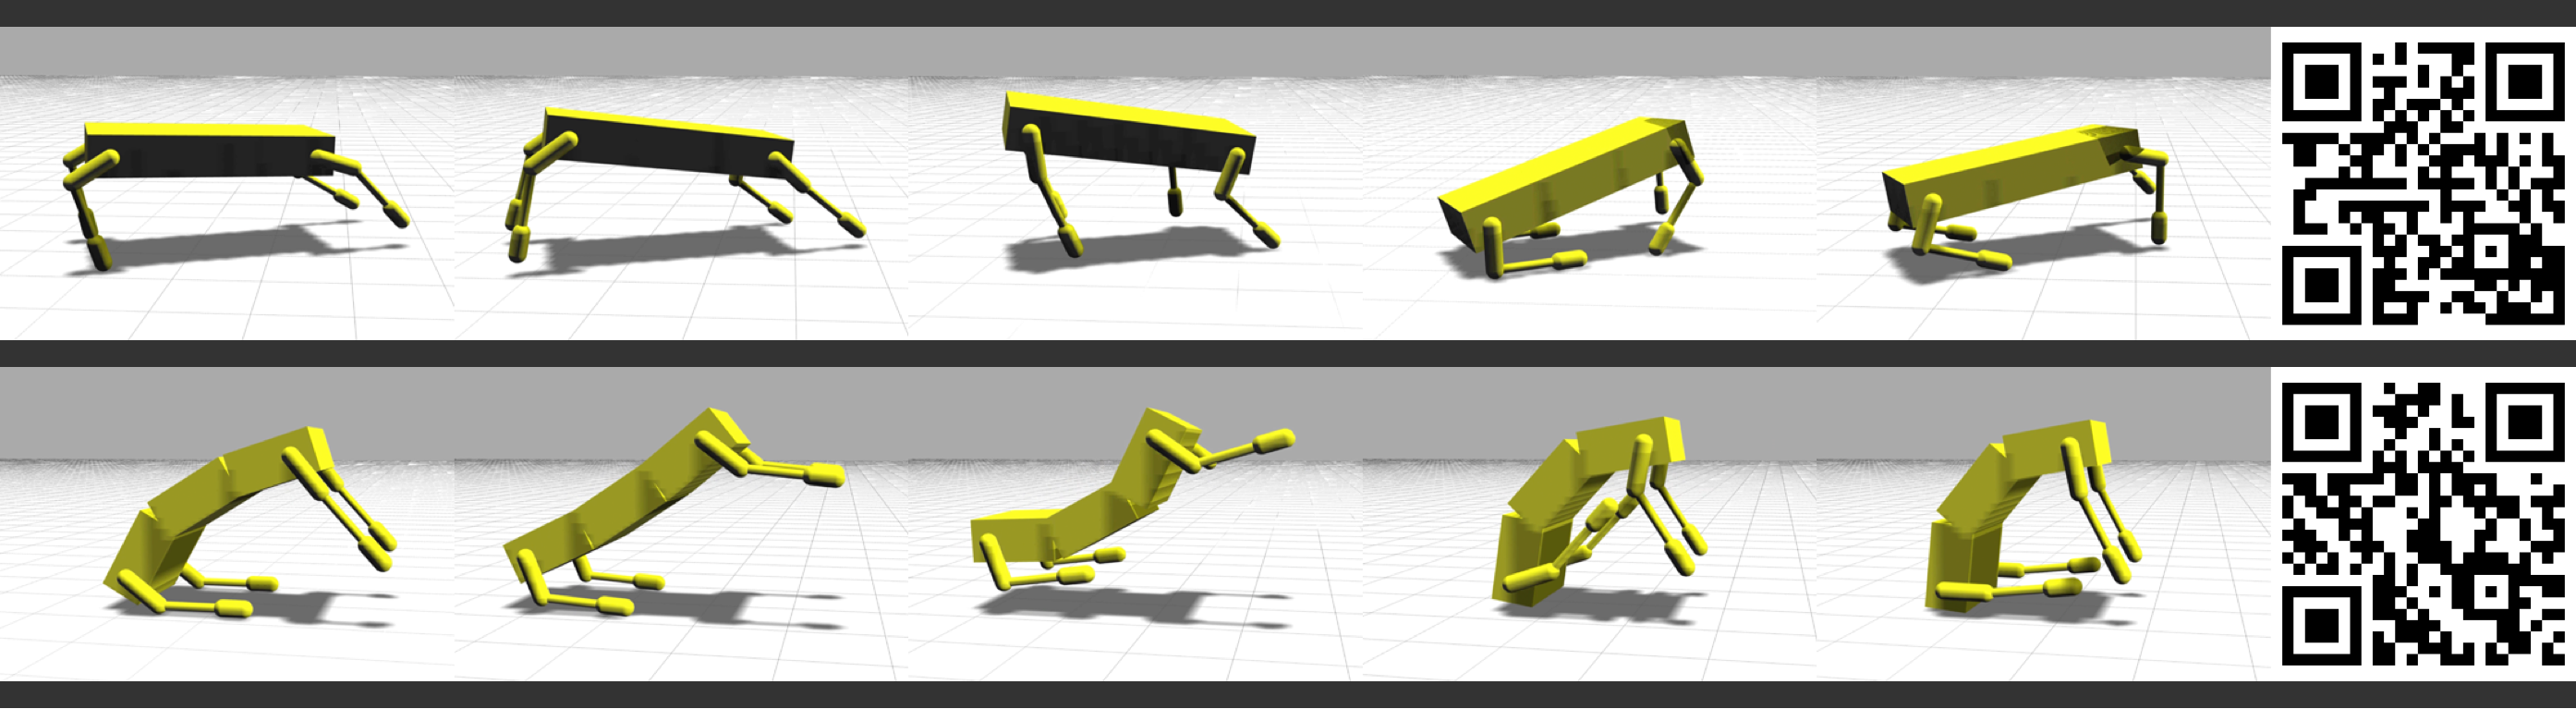
\includegraphics[width=\textwidth]{figures/quadruped.png}
\caption{Evolved gaits for a quadrupedal animat: (top) galloping, (bottom) hopping. An interactive visualization of the galloping and hopping gaits can be found, respectively, at the following links: \url{http://bit.ly/2HYXS7u} and \url{http://bit.ly/2HVY9bc}; or by visiting the links specified by the QR codes.}
\label{fig:quad_gaits}
\end{figure*}

\begin{figure*}[htb!]
\centering
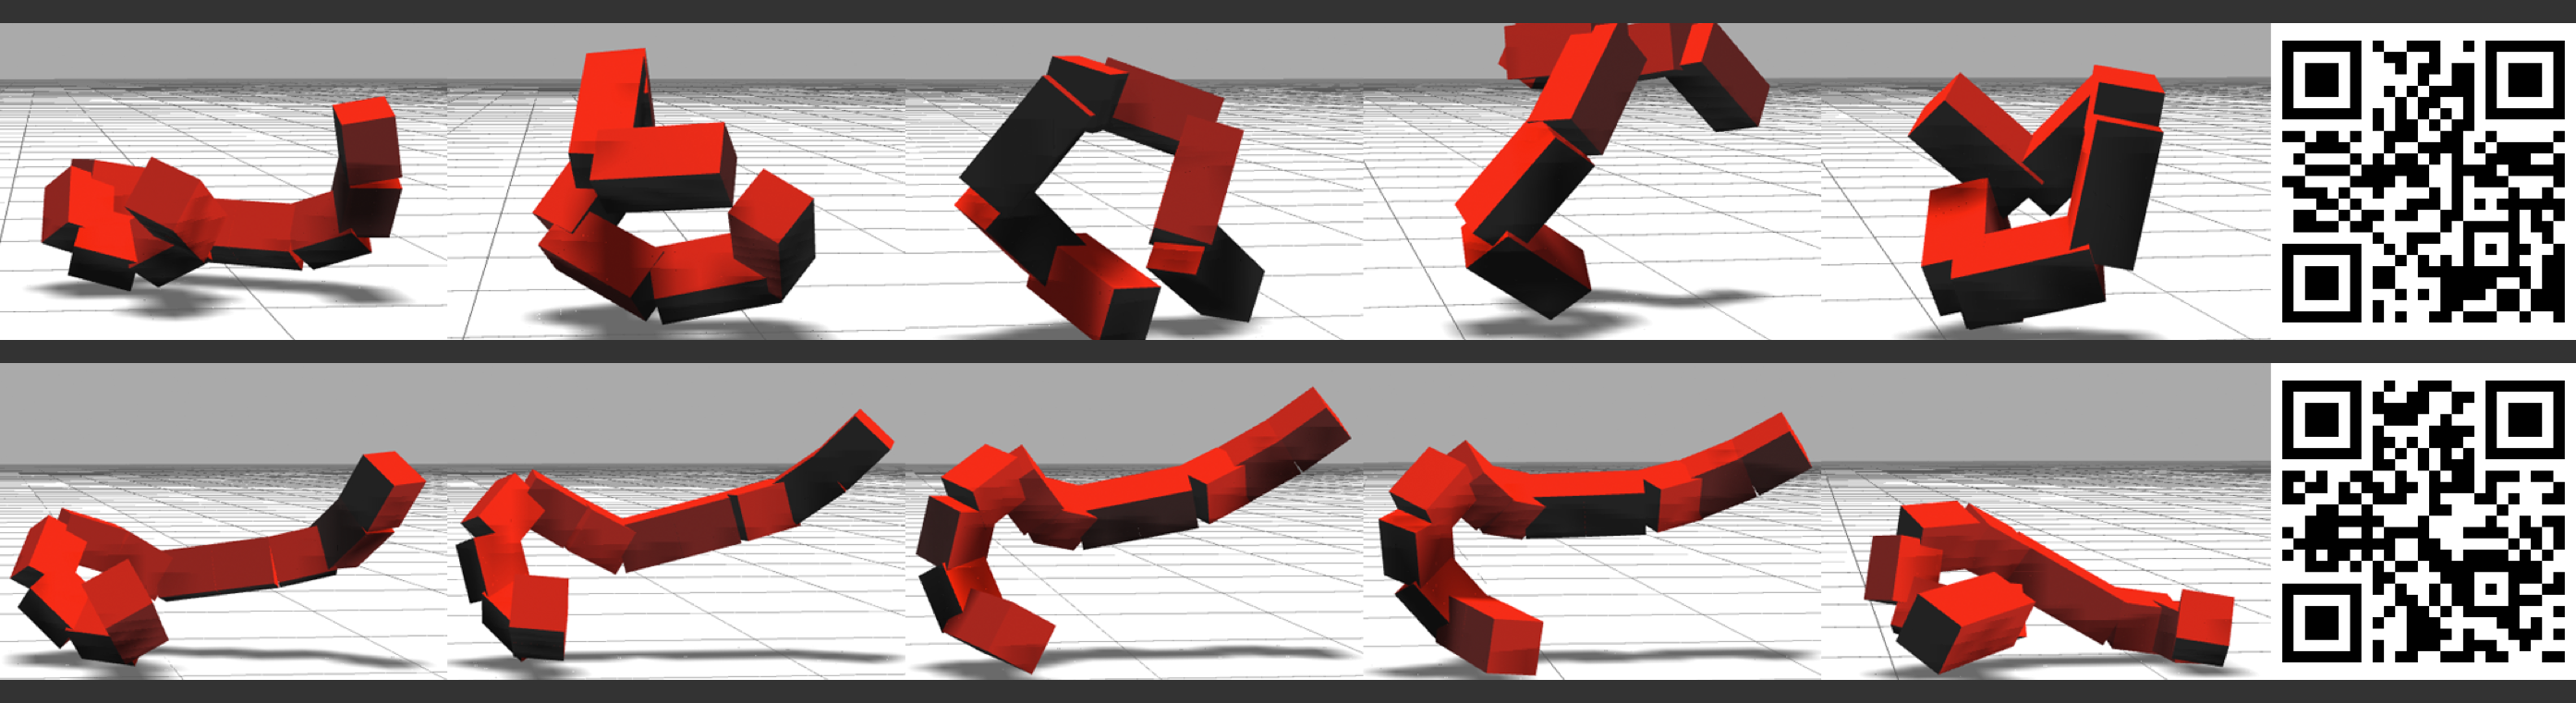
\includegraphics[width=\textwidth]{figures/worm.png}
\caption{Evolved gaits for a worm-like animat (adapted with permission from \textcite{Moore.2017.GECCO.Animat}): (top) tumbling, (bottom) hopping. An interactive visualization of the tumbling and hopping gaits can be found, respectively, at the following links: \url{http://bit.ly/2vH4Knp} and \url{http://bit.ly/2HnHa4C}; or by visiting the links specified by the QR codes.}
\label{fig:worm_gaits}
\end{figure*}


Linking to videos is a common approach to handling the problems associated with images.
%
Videos, however, are similarly static in the sense that the camera transform (viewing angles, zoom levels, etc.), object materials (colors and other material properties), and playback speed are fixed once the video is generated and uploaded.
%
Practically, this means that a viewer of the video cannot change the view angle or zoom-in on different aspects of the scene, and cannot change the color of objects if they find the chosen colors hard to see.
%
And although some web-based video players allow a viewer to speed-up/slow-down the video by small amounts, this is usually at the cost of playback smoothness; videos appear \emph{choppy} when they are slowed down since videos are recorded at a fixed frame-rate and slowing down the video effectively makes each frame appear for a longer period of time.
%
Additionally, it is common for ER researchers to generate videos by performing a video screen recording (often referred to as a screencast).
%
Since the speed of a simulation playback depends on the current load of both the CPU and GPU, recording a simulation playback via screencasting generally leads to videos with irregular frame-rates.
%
Animation software, such as Review, does not have these drawbacks.




% (3) Transition paragraph: What keen insight did you apply to overcome the shortcomings of other approaches? Structure this paragraph like a syllogism: Whereas P and P => Q, infer Q.
Review was originally developed to share visualizations among colleagues.
%
Essentially, a tool was needed to solve two common questions in evolutionary robotics: (1) how can we share behavior results without needing to generate and email (or upload) large video files, and (2) how can we enable collaborators to manipulate the scene's camera as the visualization is playing.
%
One method for achieving these two goals is to setup the same simulation and graphics environment on the machines of all collaborators, such that everyone is able to repeat the same experiment when given the same configuration (\ie{}, control and morphology parameters and environment initial conditions).
%
To ensure repeatable results, in ER research this would require all collaborators to install the same physics and graphics libraries.
%
This works for small teams and simple software packages, however, it becomes untenable when dealing with more complex systems.




% (4) Details paragraph: What technical challenges did you have to overcome and what kinds of validation did you perform?
Instead, Review has the ability to playback visualizations, inside a browser, when provided a log file.
%
Thus, the work-flow works as follows: (1) a researcher runs an evolutionary experiment (likely with the aid of a compute cluster), (2) interesting solutions are re-run, with visualization logging enabled (see section~\ref{sec:review} for details), to generate log files, (3) log files are shared with other researchers (\eg{}, via email or uploaded to a website), and (4) log files are run with Review so that everyone can see the same results.
%
Importantly, everyone using Review can independently adjust the playback speed, color of objects, and camera.



% (5) Assessment paragraph: Assess your results and briefly state the broadly interesting conclusions that these results support. This may only take a couple of sentences. I usually then follow these sentences by an optional overview of the structure of the paper with interleaved section callouts.
Review is meant to be complementary to both image sequences and videos.
%
Many researchers will not have access to the Internet while reading a research paper, and for many other cases video will suffice.
%
A web-based simulation viewer is meant for the following scenarios:

\begin{enumerate}
    \item sharing research with collaborators that need the ability to examine the scene from their own perspective, and
    \item sharing difficult-to-visualize behaviors in such a way that readers can manipulate the camera to better understand evolved behaviors.
\end{enumerate}

\section{Review}
\label{sec:review}

Due to recent advances in web technologies (\eg{}, WebGL and HTML5), web-based visualizations have become increasingly prevalent~\autocite{Evans.2014.CGJourn.Survey}.
%
Applications include: data visualization, education (\eg{}, viewing the human anatomy or the structure of a molecule), content creation (\ie{}, creating 3D models and other assets), gaming, and structure visualization (\eg{}, geospatial and architectural)~\autocite{Moore.2014.ALIFE.Web,Evans.2014.CGJourn.Survey,Mwalongo.2016.CompGraphForum.Web}.
%
The convenience of web-browsers and their increased performance has led to this increase in web-based applications.


\subsection{Usage}

Before we discuss Review in detail, we provide the following proposed usage for using Review as part of an ER study:

\begin{enumerate}
  \item Run evolutionary experiments
  \item Generate animation data (in Review log file format) for \emph{interesting} results
  \item Load animations in Review
  \item Configure the scene (change materials and environment)
  \item Export animation file (Review log file and/or glTF formats)
  \item (optional) Generate high-quality videos using glTF
  \item Share animations with other researchers
\end{enumerate}

The final step above can be achieved in several ways. First, Review log files can sent to collaborators or hosted on a professional website. In either case, the log files can automatically be fetched by Review in the following manner: https://review.github.io/?log=https://raw.githubusercontent. com/review/review.github.io/master/static/ examples/simple1.json.
%
Here, we have provided the URI of a log file to Review via an HTTP URI query component (note the "?").
%
It can often be desirable to shorten the URI with a URL shortener. For example, this link can be used in place of the previous: \url{https://goo.gl/opnkfp} (this usage is also shown in the caption of Figure~\ref{fig:passive_flex_gaits}).
%
Second, a QR Code can be generated and paired with the image sequence as shown in Figure~\ref{fig:sphere_qr}.
%
This can be useful if someone is reading a printed copy of the study in question, but they are able to visit the Review link on their smart-phone.
%
Finally, Review-based animations can be embedded into a blog-post using an HTML \textbf{iframe}.
%
This allows users to see animations in a similar manner to an embedded video, but they will be able to manipulate the viewing angle, and change the color of objects in the scene.


\begin{figure}[htb!]
    \centering

    \subfloat[Animation]{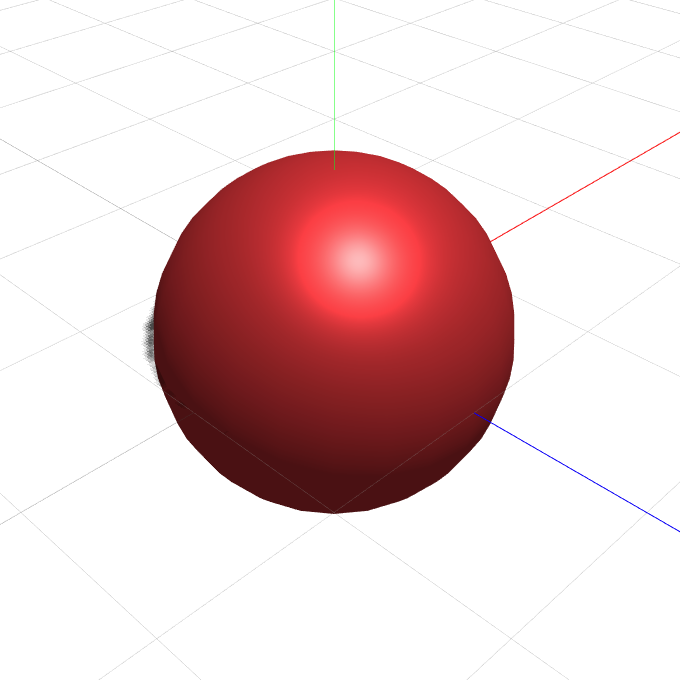
\includegraphics[width=0.25\columnwidth]{figures/sphere_ss.png}}%
    \hfil%
    \subfloat[QR Code]{
\includegraphics[width=0.25\columnwidth]{figures/sphere_qr.png}}

    \caption{(a) An image of the animation and (b) a QR Code directing a reader to the animation on Review.}
    \label{fig:sphere_qr}

\end{figure}



\subsection{Interface}


A screen-shot of the Review interface is shown in Figure~\ref{fig:review_screenshot}.
%
Review provides two methods for loading a log file (the log files is described in the next section):
(1) log files can be loaded from the local machine either by dragging the file onto the browser window, or by choosing a file from the open-file dialog box that is available when no log file is currently loaded (not shown), or
(2) log files can be specified via an HTTP URI query component and loaded automatically by Review from remote servers (as demonstrated above).


\begin{figure}[htb!]
\centering
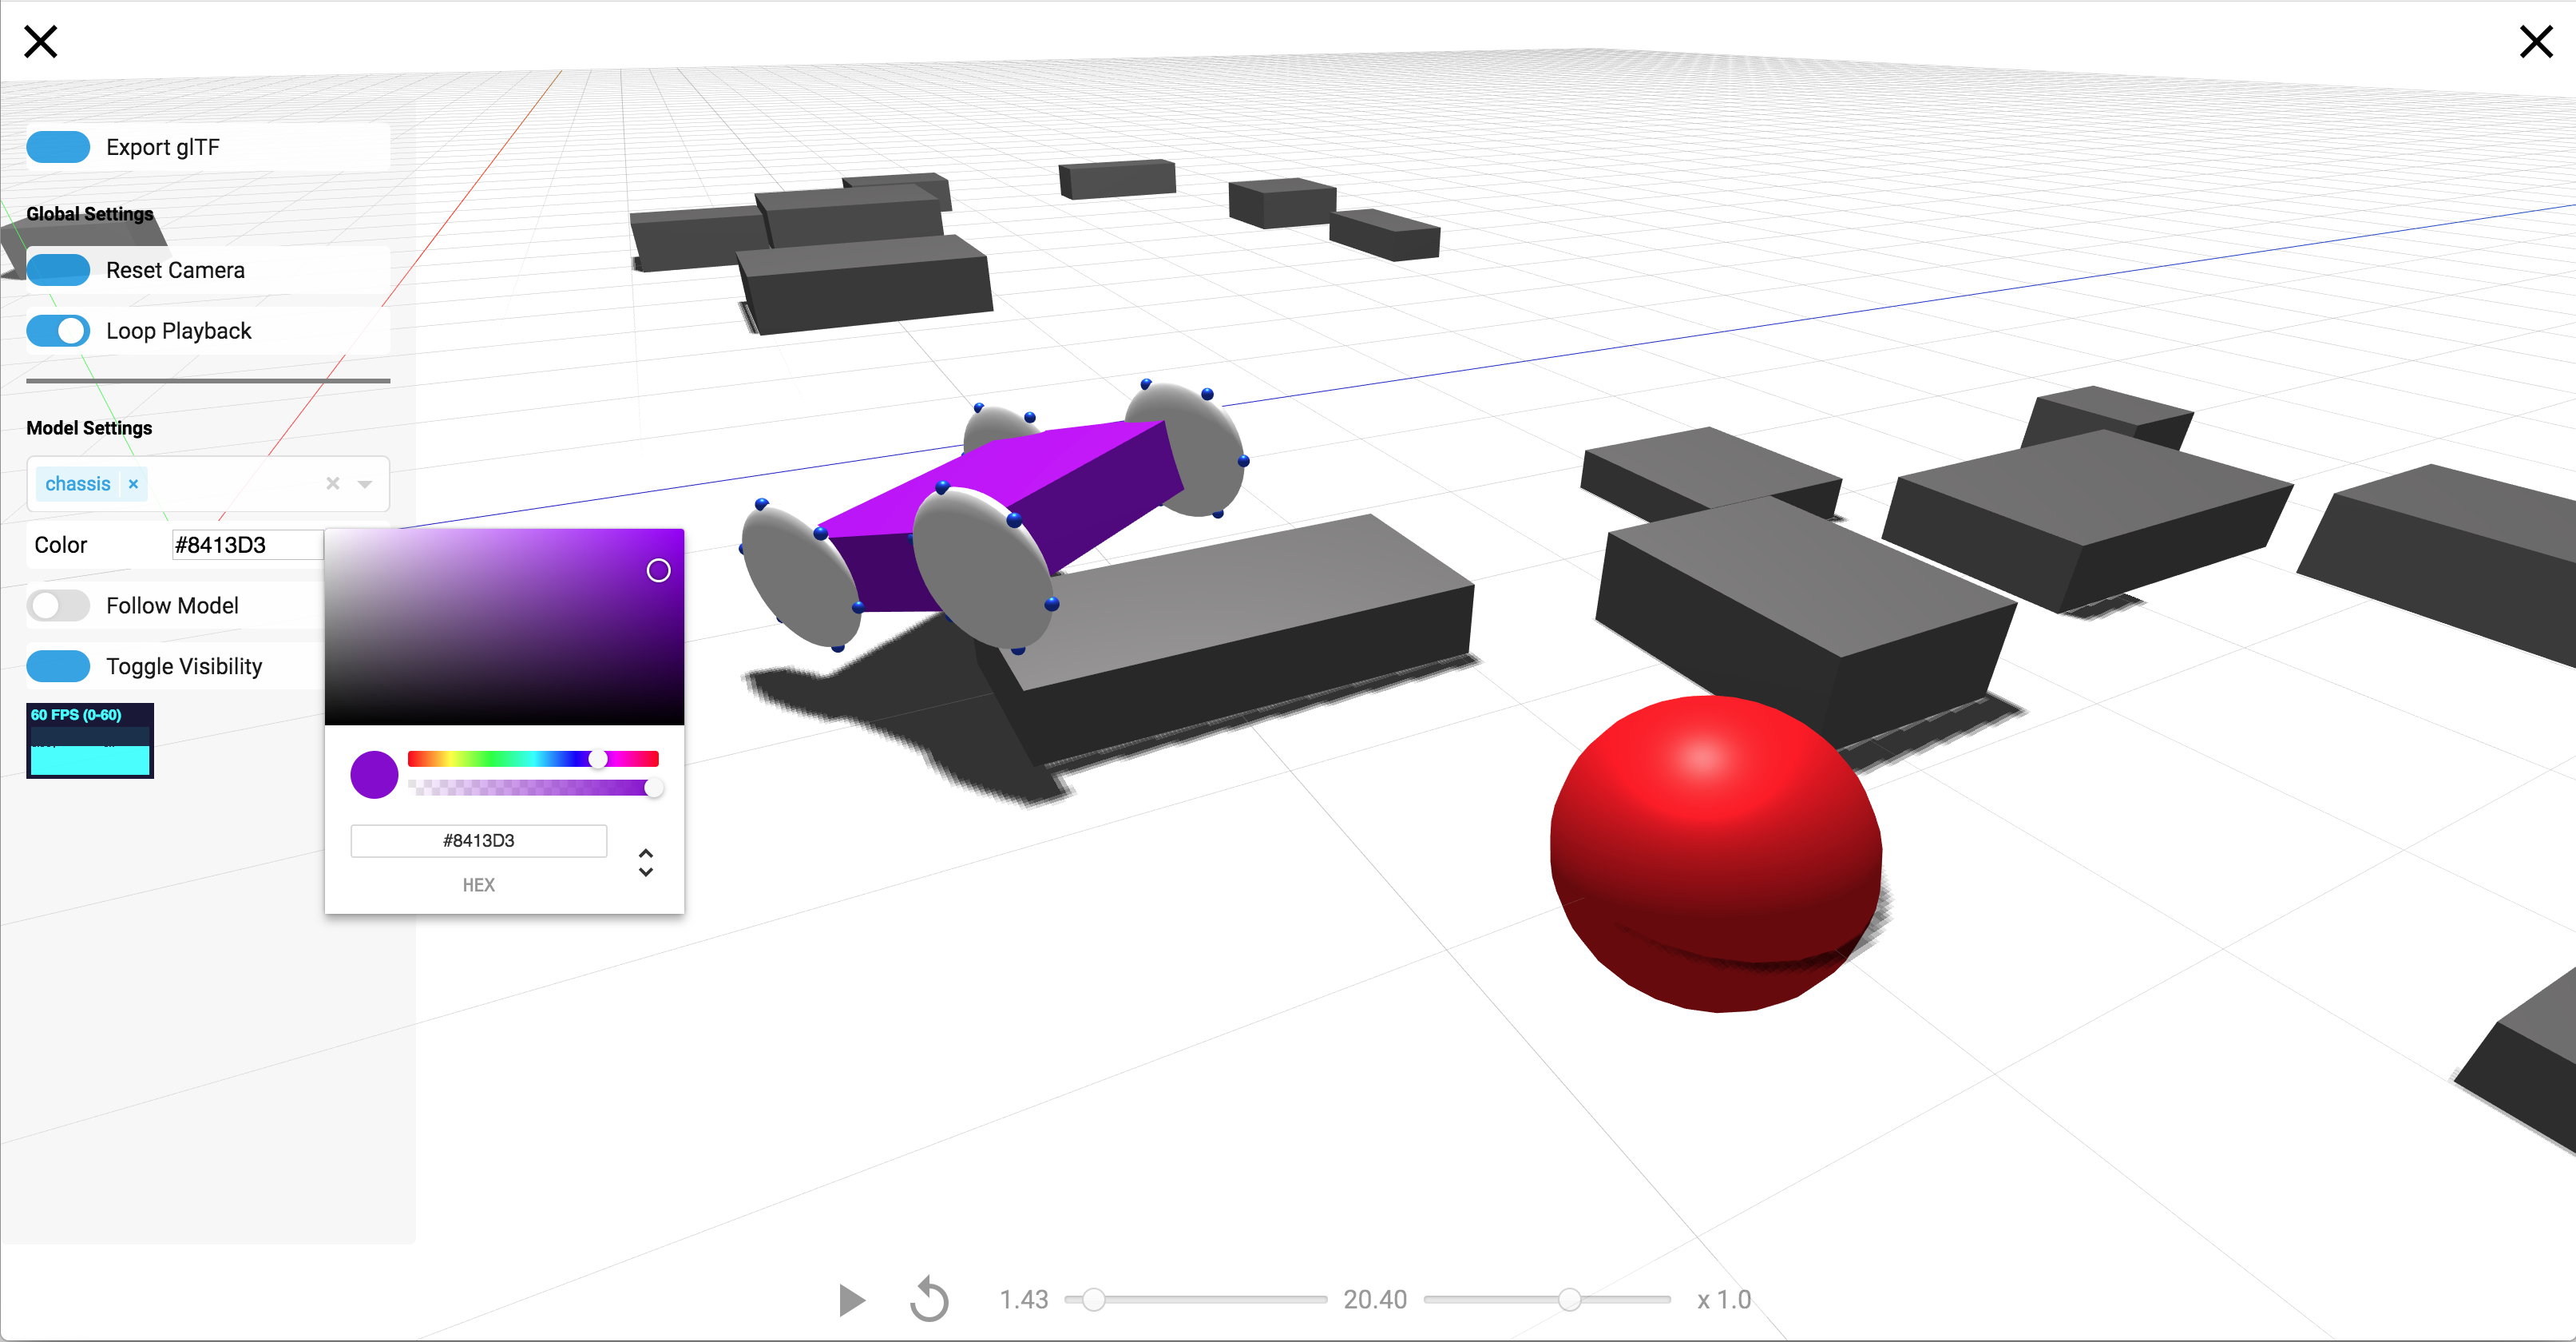
\includegraphics[width=0.9\columnwidth]{figures/review-screenshot.png}
\caption{A screen-shot of Review with a UGV simulation in progress. The color palette can be used to change the color of each object in the scene.}
\label{fig:review_screenshot}
\end{figure}


This image shows depicts a scene of a transformable wheel UGV with several obstacles, and the UGV's chassis color is currently being changed with a color picker that resides in the settings pane.
%
The settings pane can be hidden from view when it is unneeded.
%
A standard set of playback controls are available at the bottom of the screen.
%
One of the most useful controls is the progress bar, which can be \emph{scrubbed} forward and backwards. Scrubbing refers to the ability to drag the progress icon to quickly navigate through time while watching the scene update on-the-fly.
%
The playback speed can be adjusted from~\numrange{-5}{5}, where a negative number indicates that the scene will play in reverse.
%
Review also includes several other expected features, for example, the ability to following a specific object with the camera and to reset the camera to its original settings.




\subsection{Log File Format}

One motivating factor for developing Review was the lack of an alternative with a suitable file format.
%
Most similar tools (described in section~\ref{sec:related_work}) require a complex file format that is difficult to generate alongside a physical simulation--likely because most tools anticipate that visualization data is being generated by an authoring tool like Blender\footnote{\url{https://www.blender.org/}} or Autodesk Maya\footnote{\url{https://www.autodesk.com/products/maya/overview}}.
%
The Review file format was specifically designed to be easily generated while running a simulation. An example of the Review log file format follows:

\begin{minipage}{\linewidth}
\begin{lstlisting}[style=json]
{
  "name": "Sphere Example",
  "timeStep": 0.25,
  "objects": [{
    "name": "sphere1",
    "mesh": "sphere"
  }],
  "frames": [
    { "sphere1": { "t": [0, 0, 0] } },
    { "sphere1": { "t": [1, 0, 0] } },
    { "sphere1": { "t": [1, 0, 1] } },
    { "sphere1": { "t": [0, 0, 1] } },
    {  },
    { "sphere1": { "t": [0, 0, 0] } }
  ]
}
\end{lstlisting}
\end{minipage}

Click the following link to interact with this animation: \url{https://goo.gl/9ZUYYe}.
%
This is a visualization of a sphere that moves in a square pattern and pauses for one frame when it reaches its position at the fourth frame.


The log file is a JSON file with a specific schema~\autocite{JSON.2018.Schema}. Here we describe a basic file, but the full schema can be found in the Review Git repository.
%
This file format is human readable and writable, and nearly all programming languages include a library for manipulating JSON data.
%
The Review logging library\footnote{\url{https://github.com/review/logger-cpp}} used to generated the  files linked in this study has been provided, and it contains less than 100 lines of C++ code and has only one external dependency (a C++ JSON library).
%
This format has four required fields. The \textbf{name} (string) and \textbf{timeStep} (number) provide a unique name for the visualization and the time elapsed between frames, respectively.


\textbf{objects} (array) is a list of all objects that are present in the scene. In the example, there is only one object and only the required object fields are specified.
%
Each object must have a unique \textbf{name} (string) and a \textbf{mesh} (string).
%
The \textbf{mesh} value denotes either a primitive (\emph{cube}, \emph{cylinder}, or \emph{sphere}) or a URI to an external resource (\eg{}, an STL or COLLADA file).
%
In addition to these fields, several other attributes can be specified. The most prominent fields include: a physically based rendering (PBR) material, translation, rotation, and scale.


\textbf{frames} (array) is a list of all frames in the scene, and the time lapsed between each pair of consecutive frames is always \textbf{timeStep}.
%
Each frame is a JSON object where the keys (left side of the colon) denote objects named in the \textbf{objects} array, and the values (right side of the colon) denote object transformations.
%
In the example, the only attribute of \emph{sphere1} that changes is its translation. The most common animation attributes are translation (\textbf{t}) and rotation (\textbf{r}), but other types can be specified (\eg{}, color).
%
As exemplified by the fifth frame, this log file format enables some frames to not include any transformations. This greatly reduces the file size when many objects are in the scene but only a few are in motion at any given time.
%
For example, for the UGV visualization in Figure~\ref{fig:review_screenshot} all 30 boxes are dynamic, but only one or two boxes are pushed by the UGV in any given frame.
%
Although frame data may be omitted, currently the frames themselves must be present (even if empty) to ensure that the duration of the simulation is accurate--the log file format does not currently allow for variable \textbf{timeSteps} between different frames.



\subsection{Details}

After Review loads a JSON-format log file, it converts it into glTF~2.0\footnote{\url{https://github.com/KhronosGroup/glTF}}.
%
glTF is a transmission format specified in JSON that is used for loading and saving 3D models and scenes.
%
The Review log format is converted into glTF because glTF is supported by nearly all rendering software and authoring tools.
%
In our early implementations of Review, we were using the Review log files directly, however, by converting to glTF we can rely on well-tested and optimized animation frameworks for visualizing robot behaviors.
%
Thus, Review maintains the benefit of a simple file format while also gaining the capabilities of more capable rendering libraries.


Specifically, Review uses three.js~\autocite{Cabello.2013.ThreeJS} to render animated scenes to the screen.
%
three.js includes a modern rendering pipeline, great support for animations, and can import glTF files.
%
Perhaps the most important feature of the three.js animation system is \emph{interpolation}, whereby three.js will interpolate transformation between frames.
%
In the moving sphere example above, the time between frames is 0.25s, however, most computers will have no trouble rendering the scene at 60 frames-per-second, which means that three.js will use interpolation to generate roughly 15 frames in-between each frame.
%
The impact of interpolation is most dramatic when the playback speed is reduced. For instance, when the playback speed is set to 0.25 three.js generates 60 interpolated frames, thereby providing a smooth animation.
%
Without interpolation, animations would be choppy (similar to a slowed-down video).

\section{Related Work}
\label{sec:related_work}

Although web-based visualizers can be found for many different domains, there are only a few that have similar capabilities to those we describe here--namely, sharing animations with other collaborators and other researchers.
%
\url{Clara.io}~\autocite{Clara.2018.SIGGRAPH.Web} is a cloud-based web-application for modeling, animating, and rendering scenes.
%
Clara.io has an impressive list of features, including the ability to create models and scenes in the browser. With Clara.io you can send animation links to collaborators, but the data files must be hosted by Clara.io and the project is not open source.
%
More importantly, Clara.io uses standard graphics formats, which makes it difficult to generate animation data as part of an evolutionary experiment work-flow.
%
Sketchfab~\autocite{Sketchfab.2018.Web} is another alternative, and like Clara.io, Sketchfab hosts the data files and works with common graphics files.
%
While both of would enable the sharing of visualizations, both would require an extensive amount of work to generate visualization data.
%
Another drawback of these websites is that they require a paid account to keep any files private, whereas with Review a researcher can choose to only share the log files with specific collaborators.

\section{Conclusions}
\label{sec:conclusions}

In this paper we have presented Review, a web-based tool for sharing evolutionary robotics visualizations with collaborators and other researchers.
%
The interactive visualizations enabled by Review are complementary to current techniques such as providing image sequences and links to videos.
%
Moreover, the simple log file format and export to glTF feature will enable researchers to import their simulation results into 3D author tools such as Maya, which will enable the production of high-quality videos more suitable for presentations.
%
In the future, we anticipate adding the following features: (1) the ability to import more than one animation at a time so that researchers can compare the results from different trials in the same view, (2) support for additional mesh and material formats, and (3) the ability to generate videos.

\begin{acks}

The authors would like to thank the contributions of Dr. Razib Iqbal, Michael Brattin, Kyle Finter, Garren Ijames, Brett Spatz, and Jesse Stewart from Missouri State University.

\end{acks}


\printbibliography


\end{document}
